\documentclass[a4paper,12pt,twoside]{article}
\usepackage{amsmath}
\usepackage{amssymb}
\usepackage{bm}
\usepackage{booktabs}
\usepackage[small,bf]{caption}
\usepackage{comment}
\usepackage{cuted}
\usepackage[shortlabels]{enumitem}
\usepackage{fancyhdr}
\usepackage{fancybox}
\usepackage{float}
\usepackage[T1]{fontenc}
\usepackage[a4paper,left=1in,right=1in,top=0.25in,bottom=1in,
    headheight=76.33466pt,
    headsep=\dimexpr1in-62.33466pt\relax,
    includehead
]{geometry}
\usepackage{graphicx}
\usepackage{hyperref}
\usepackage[utf8]{inputenc}
% \usepackage{lipsum}
% \usepackage{listings}
\usepackage{minted}
\usemintedstyle{emacs}
\usepackage{multirow}
\usepackage{parskip}
\usepackage{ragged2e}
\usepackage{setspace}
\usepackage{soul}
% \onehalfspacing
\usepackage{subcaption}
% \usepackage[subrefformat=parens,labelformat=parens]{subfig}
\usepackage{tabularx}
% \usepackage{titling}
\usepackage{xurl}
\usepackage{biblatex}
\addbibresource{Lab2.bib}
\usepackage{background}
\backgroundsetup{contents=
\includegraphics{waterprint.jpg}, scale=0.8, opacity=0.1}
\pagestyle{fancy}
\fancyhf{}
\fancyhead[LE,RO]{}
\fancyhead[CE,CO]{
\includegraphics[width=0.7\textwidth]{JILogo.png}}
\fancyhead[RE,LO]{}
\fancyfoot[CE,CO]{\leftmark}
\fancyfoot[CE,CO]{\thepage}
\lfoot{\textit{ECE4810J \textbf{SoC Design} | Fall 2022}}
\renewcommand{\headrulewidth}{1pt}
\renewcommand{\footrulewidth}{1pt}
\definecolor{caption2color}{HTML}{2e5395}
\hypersetup{
    colorlinks=true,
    linkcolor=blue,
    filecolor=magenta,      
    urlcolor=cyan,
    pdfpagemode=FullScreen,
}

\author{Xinfei Guo, Yihua Liu}
\title{ECE4810J FA2021\\ \small Lab \#1}
\date{September 19, 2022}

\begin{document}
% \maketitle
\thispagestyle{fancy}

\begin{center}
    \vspace*{0pt}
    \Large{\textbf{ECE4810J SoC Design}}\\
    \vspace*{2pt}
    \large{Fall 2022}\\
    \vspace*{10pt}
    \Large{\textcolor{caption2color}{Lab \#2 Design with High Level Synthesis on Arty Z7 SoC Development Platform}}\\
    \normalsize{\hl{Due: 11:59pm Oct. 9th, 2022}}
    \rule[-5pt]{.97\linewidth}{0.05em}
\end{center}

\textbf{Logistics:}
\begin{itemize}
    \item This lab is a team exercise.
    \item Please use the discussion board on Piazza for Q\&A.
    \item All reports and code (if available) MUST be submitted to the assignment of Canvas.
    \item Internet usage is allowed and encouraged.
    \item No late submission is allowed for this lab.
\end{itemize}
\tableofcontents
\section{Overview}
In this lab, you will go through two exercises to create designs with high-level synthesis languages (instead of strict hardware description languages like Verilog/VHDL/SystemVerilog) and PYNQ. The goals of this lab are to
\begin{itemize}
    \item Get familiar with the concept of High-level Synthesis (HLS)
    \item Learn to use HLS to create an IP block in C/C++
    \item Learn about differences between programming with HLS vs. Verilog in terms of design quality
    \item Get started with the Arty Z-7 board as a Python accelerator and be able to run example Jupyter notebooks with the board
    \item Load PYNQ overlays, use overlays and create overlays
\end{itemize}
\section{Create and Use Custom IP Blocks Using High-Level Synthesis}\label{S2}
There are a number of reasons why High-Level Synthesis (HLS) tools have been developed. Most of all, it has to do with developer productivity and code reuse, as well as other business-related reasons. RTL development in hardware description languages such as Verilog and VHDL is slow and difficult to debug, verify, and update. Moreover, it can not be done by software engineers without intense training in hardware development. These translate into a high expense for businesses. High-level synthesis attempts to partially solve this problem, by generating HDL code from a higher-level language such as C/C++. Further hardware control is enabled by the use of HLS PRAGMAS. Designs made using HLS are typically not the most optimal possible solutions, even after several optimizations, but are often considered acceptable considering the low engineering cost (NRE) and the throughput gains.

In this part of the lab, we will only get started with HLS, by reimplementing the 16-bit multiplier using C++ and HLS to generate the AXI-Lite slave IP block.
\subsection{Creating the Vitis HLS project}
\begin{enumerate}
    \item Open Vitis HLS->PROJECT->Create Project.
    \item Call the project hls\_multiplier and locate it in your group’s working folder.
    \item Similarly, in the Top Function field, write hls\_multiplier. The Top Function is the C/C++ function that will be translated to HDL by the HLS algorithm. If it calls other functions, they will also be translated to HDL. Skip Add/Remove Testbench Files.
    \item Leave the Solution Name as default, the Period is 10 ns since the board frequency is 100 MHz, and for the Part Selection, please select xc7z020clg400-1 of Family Zynq-700, Speed = -1, Flow Target set to be Vivado IP Flow Target. You will notice that Vitis HLS looks less “busy” compared to Vivado. This is because Vivado HLS only simulates, synthesizes, and packages the IP block, but does not interface with the hardware directly. The output from Vitis HLS is to be later imported into a Vivado project. Let's add the necessary code to implement and test the HLS multiplier AXI Lite slave IP block.
    \item In the Explorer, right-click on Source and click Add Source File... Add lab2\_starter/\\
    hls\_multiplier.cpp. The code is really simple. The hls\_multiplier C++ function takes in two unsigned short int arguments $a$ and $b$, 16-bits each, and returns an unsigned int which is 32-bit. Inside, the product $p$ is declared as a 32-bit unsigned int, is given the value $a\times b$ and is returned. The \texttt{\#pragma HLS INTERFACE} lines specify that the interface to be used is a slave AXI Lite and are all into the same bundle.
    \item In the Explorer, right-click on Test Bench and click Add Test Bench File... Add lab2\_starter/test\_hls\_multiplier.cpp. Again, the code is very straightforward - please read it and understand what is going on.
\end{enumerate}
\subsection{Testing the hls\_multiplier and exporting the IP block}
Vitis HLS offers a few ways to test your design, both as C Simulation and as C/RTL Cosimulation. To start a simulation - use the comfortably ordered buttons on the top area.
\begin{enumerate}
    \item Project menu->Index C source.
    \item Project menu->Run C Simulation or click the black triangle button next to the green triangle button, click C Simulation. In the pop-up C Simulation Dialog, you can check Clean Build in the Options frame. Click OK. Observe the Vitis HLS Console. After the C simulation is finished, hls\_multiplier\_csim.log will pop up, showing:
    \begin{minted}[breaklines]{text}
INFO: [SIM 2] *************** CSIM start ***************
INFO: [SIM 4] CSIM will launch GCC as the compiler.
   Compiling ../../../../lab2_starter/test_hls_multiplier.cpp in debug mode
   Compiling ../../../../lab2_starter/hls_multiplier.cpp in debug mode
   Generating csim.exe
initialized variables: a=2, b=3, p=0 
testing hls_multiplier: 2 * 3 = 6 
INFO: [SIM 1] CSim done with 0 errors.
INFO: [SIM 3] *************** CSIM finish ***************
    \end{minted}
    \item Solution menu->Run C Synthesis->Active Solution or click the black triangle button next to the green triangle button, click C Synthesis. You can keep default settings in the pop-up dialog C Synthesis - Active Solution. This step starts the translation of the C/C++ code to HDL (both Verilog and VHDL), synthesizes it for the targeted chip and the targeted frequency, and generates a report. After the synthesis is finished, you can observe "Finished C synthesis" in Vitis HLS Console and view the Synthesis Summary Report of 'hls\_multiplier' in the pop-up tab Synthesis Summary(solution1). Read the Timing Estimate and Performance \& Resource Estimates section especially. Note that the organization of the report is very different from those generated by previous versions of Vitis HLS (or originally Vivado HLS).
    \begin{figure}[H]
        \centering
        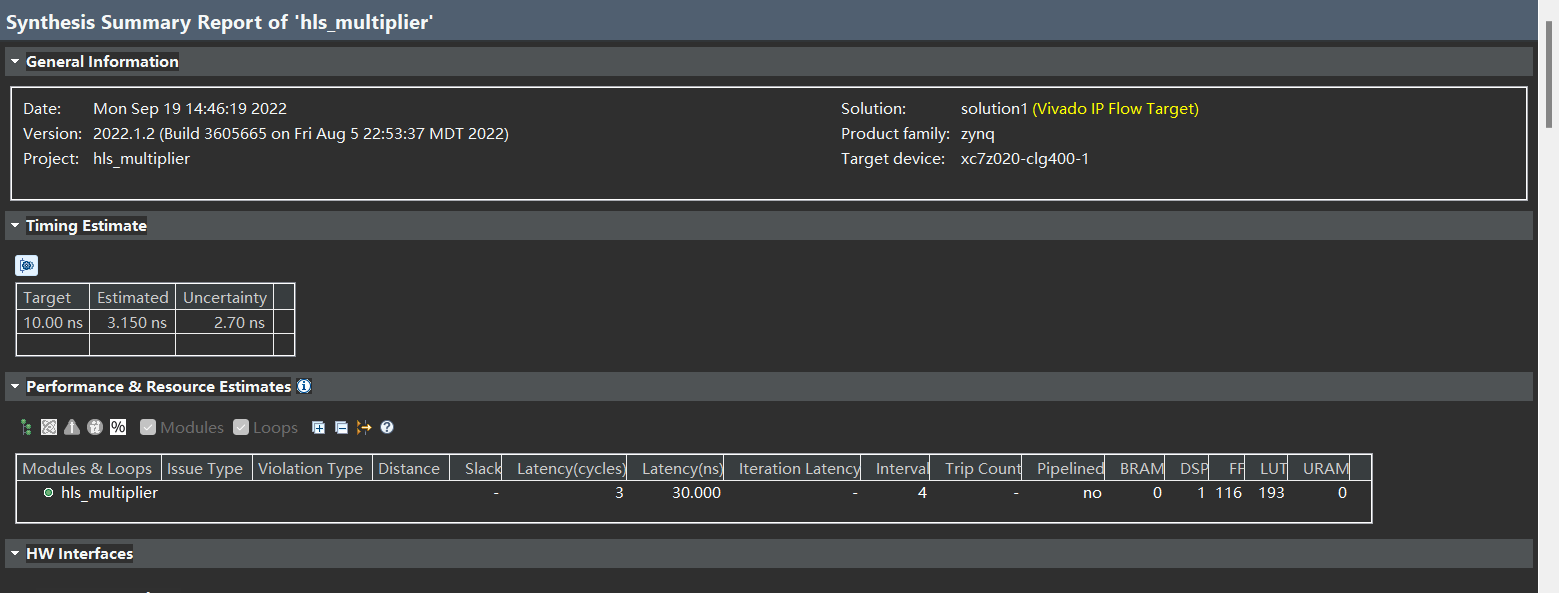
\includegraphics[width=\textwidth]{images/1.png}
    \end{figure}
    \item Now that everything seems reasonable at the C Simulation level and at the C Synthesis level, click the black triangle button next to the green triangle button, click Cosimulation or run Flow Navigator->C/RTL COSIMULATION->Run Cosimulation. Use the default settings in the Co-simulation Dialog (Vivado XSIM, Verilog). It does the simulation of both the C and the generated RTL and compares the final results, and ensures that they match. After the cosimulation finished, Vitis HLS Console outputs:
    \begin{minted}[breaklines]{text}
INFO: [Common 17-206] Exiting xsim at Mon Sep 19 15:12:00 2022...
INFO: [COSIM 212-316] Starting C post checking ...
initialized variables: a=2, b=3, p=0 
testing hls_multiplier: 2 * 3 = 6 
INFO: [COSIM 212-1000] *** C/RTL co-simulation finished: PASS ***
INFO: [COSIM 212-211] II is measurable only when transaction number is greater than 1 in RTL simulation. Otherwise, they will be marked as all NA. If user wants to calculate them, please make sure there are at least 2 transactions in RTL simulation.
INFO: [HLS 200-111] Finished Command cosim_design CPU user time: 1 seconds. CPU system time: 0 seconds. Elapsed time: 18.82 seconds; current allocated memory: 0.000 MB.
INFO: [HLS 200-112] Total CPU user time: 7 seconds. Total CPU system time: 1 seconds. Total elapsed time: 24.436 seconds; peak allocated memory: 1.537 GB.
Finished C/RTL cosimulation.
    \end{minted}
    In the generated Cosimulation Report for 'hls\_multiplier' in the pop-up tab Co-Simulation Report(solution1), you are expected to see Status: \textcolor{green}{Pass} - which means the test was successful. Now that all these tests passed, it's time to export the design to an IP block.
    \begin{figure}[H]
        \centering
        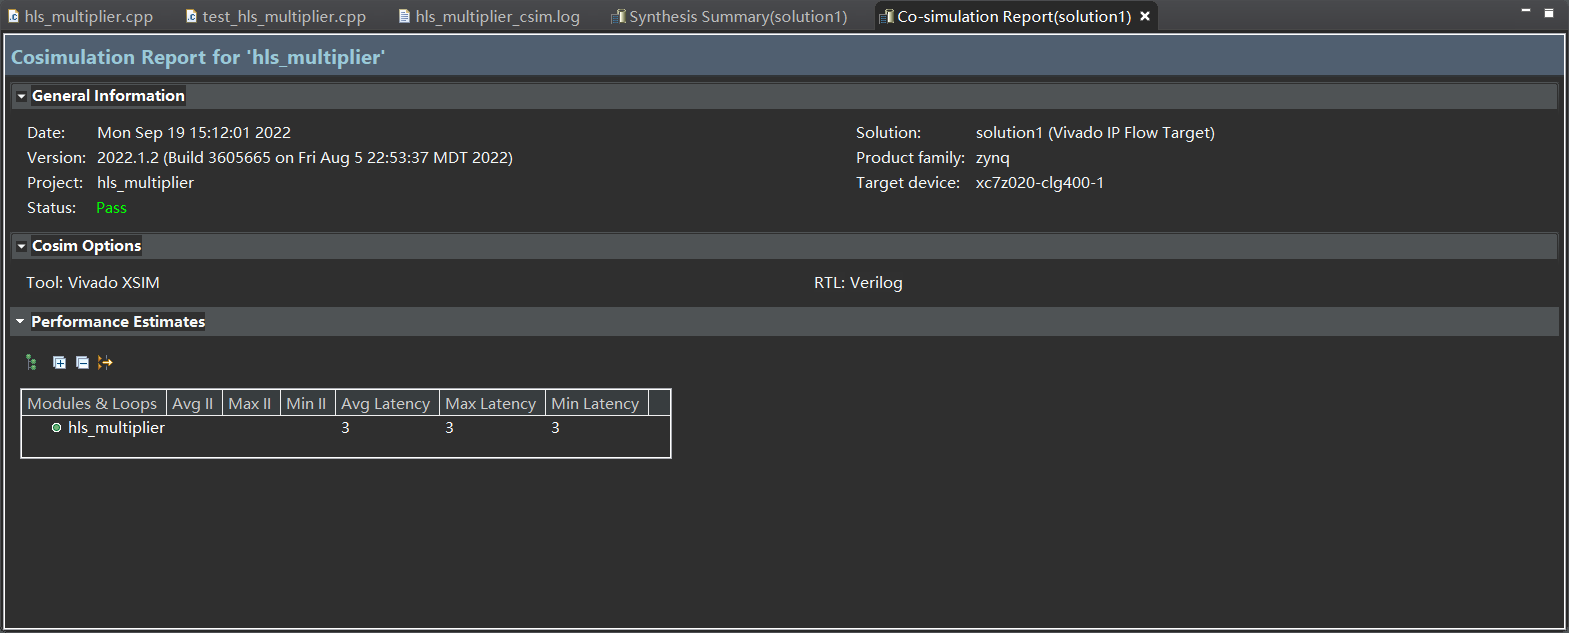
\includegraphics[width=\textwidth]{images/2.png}
    \end{figure}
    \item Solution menu->Export RTL or click the black triangle button next to the green triangle button, click Export RTL. In the pop-up dialog Export RTL, choose the Output Location, then click OK. Wait until Vitis HLS Console shows "Finished Export RTL/Implementation". You can now close Vivado HLS.
\end{enumerate}
\subsection{Adding the hls\_multiplier AXI Lite Slave IP Block to your Vivado design}
\begin{enumerate}
    \item Open your Vivado project for Lab 1 or create a new Vivado project and create the Zynq\_CPU block design with a ZYNQ7 Processing System and its HDL wrapper. In Tools->Settings->Project Settings->IP->Repository. Add the hls\_multiplier/\\
    solution1/impl/ip directory. This will allow Vivado to find the IP we just created using Vitis HLS. If you have not add the rtl\_multiplier\_v1.0 IP, also add the ip\_repo/rtl\_multiplier\_1.0 directory.
    \item Next, in the Block Design, click on Add IP and search for the Hls\_multiplier. Add it to your design. If you have not add rtl\_multiplier\_v1.0 IP, also add rtl\_multiplier\_v1.0. Run Connection Automation to automatically have it connected to the AXI Interconnect.
    \item Save all files and click on Generate Bitstream to (re-)run Synthesis and Implementation over the (updated) design. Check the resource utilization and look over the implementation. In the following image, the hls\_multiplier area is highlighted yellow, while the rtl\_multiplier area is highlighted red. To highlight hls\_multiplier\_area and rtl\_multiplier area, Open Implemented Design, in the Netlist tab, choose\\
    Zynq\_CPU\_wrapper->Zynq\_CPU\_i (Zynq\_CPU), right click hls\_multiplier\_0 (Zynq\_CPU\_hls\_multiplier\_0\_0) and rtl\_multiplier\_0 (Zynq\_CPU\_rtl\_multiplier\_0\_0), select "Highlight Leaf Cells"->Default/Color 2 and Color 7 respectively. Note that the resource utilization images in the Device window generated by different people are different. Example results are shown below.
    \begin{figure}[H]
        \centering
        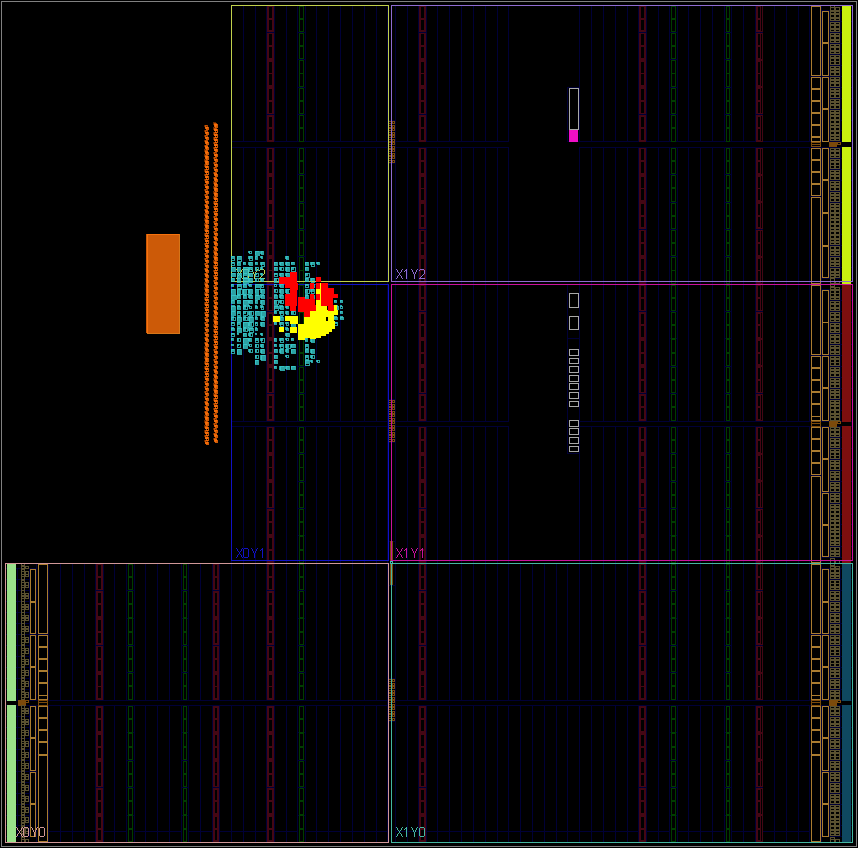
\includegraphics[width=\textwidth]{images/3.png}
    \end{figure}
\end{enumerate}
\subsection{Interfacing with the RTL and HLS blocks in Software}
\begin{enumerate}
    \item As what has been practiced in Lab\#1, Export Hardware... as\\
    Zynq\_CPU\_wrapper\_hw\_platform\_4.xsa and Launch Vitis.
    \item Create a new application called hello\_hls\_rtl\_multiplier starting with the Hello World template.
    \item Right-click Explorer->hello\_hls\_rtl\_multiplier\_system->hello\_hls\_rtl\_multiplier->src, click Import Sources to replace helloworld.c with lab2\_starter/hls\_rtl\_multiplier.c through right. The first part of this code does the same as before, testing the rtl\_multiplier in Lab \#1. The second part of the code tests the hls\_multiplier. Vitis HLS generates not only an HDL implementation of the IP block but also functions that enable the user to use the IP block correctly. Make sure you understand the code.
    \item Build and run the code on the Arty Z-7 board. The result from the Vitis Serial Terminal is shown below:
    \begin{figure}[H]
        \centering
        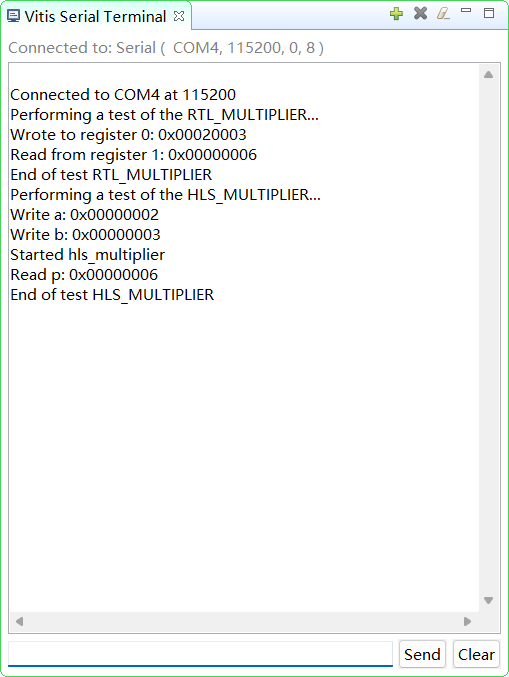
\includegraphics[width=\textwidth]{images/4.png}
    \end{figure}
\end{enumerate}
\subsection{Follow-up Exercises}
In this task, you are required to implement a 32-bit ALU (Arithmetic Logic Unit), i.e. a block that can perform operations defined in RV32IM (RISC-V 32-bit Base Integer Instruction Set Version 2.1 + “M” Standard Extension for Integer Multiplication and Division Version 2.0) \cite{riscv-unpriv}:
\begin{table}[H]
    \centering
    \begin{tabular}{|c|c|c|}
        \hline
        Operation & Code & Selector ID \\
        \hline
        Add & ALU\_ADD & 0 \\
        \hline
        Subtract & ALU\_SUB & 1 \\
        \hline
        Set less than & ALU\_SLT & 2 \\
        \hline
        Set less than (unsigned) & ALU\_SLTU & 3 \\
        \hline
        And & ALU\_AND & 4 \\
        \hline
        Or & ALU\_OR & 5 \\
        \hline
        Exclusive or & ALU\_XOR & 6\\
        \hline
        Shift left (logical) & ALU\_SLL & 7 \\
        \hline
        Shift right (logical) & ALU\_SRL & 8 \\
        \hline
        Shift right (arithmetic) & ALU\_SRA & 9 \\
        \hline
        Multiply & ALU\_MUL & 10 \\
        \hline
        Multiply (upper XLEN bits, signed$\times$signed) & ALU\_MULH & 11 \\
        \hline
        Multiply (upper XLEN bits, signed$\times$unsigned) & ALU\_MULHSU & 12 \\
        \hline
        Multiply (upper XLEN bits, unsigned$\times$unsigned) & ALU\_MULHU & 13 \\
        \hline
        Divide & ALU\_DIV & 14 \\
        \hline
        Divide (unsigned) & ALU\_DIVU & 15 \\
        \hline
        Remainder & ALU\_REM & 16 \\
        \hline
        Remainder (unsigned) & ALU\_REMU & 17\\
        \hline
    \end{tabular}
    \caption{RV32IM ALU Operations.}
\end{table}
Based on lab2\_starter/rtl\_alu.sv, create and package a new IP \texttt{rtl\_alu} in Vivado. In this part, you only need to complete the rtl\_alu module. Suppose you have two 32-bit inputs, one 5-bit input, and one 32-bit output, you will need four registers, which are specified when you add AXI interfaces during the "Create and Package New IP" process. In Vitis HLS, create a new project \texttt{hls\_alu} with source hls\_alu.cpp and test bench test\_hls\_alu.cpp. In the test bench, test the functional correctness of all 18 operations. Run C simulation and take a screenshot of hls\_alu\_csim.log; run C synthesis and take a screenshot of the Timing Estimate and Performance \& Resource Estimates in the Synthesis Summary Report; run cosimulation and take a screenshot of the Cosimulation Report.

Add rtl\_alu and hls\_alu to the block design. Create an HDL wrapper and generate the bitstream. Take a screenshot of the Device highlighting rtl\_alu and hls\_alu leaf cells and screenshots of the Summary in the Utilization report and the Design Timing Summary in the Timing report in your Implemented Design. Pay attention to whether there are latches. Compare the rtl\_alu and hls\_alu and summarize any differences you observed. Then, export hardware as Zynq\_CPU\_wrapper\_hw\_platform\_5.xsa.

Create a Vitis application project named hello\_hlr\_rtl\_alu from the Hello World template and import the hardware. Replace helloworld.c with hls\_rtl\_alu.c. In the project, test all 18 operations of both rtl\_alu and hls\_alu. Take a screenshot of your Vitis IDE window at the build-finished state and a screenshot of the output in the Vitis Serial Terminal.

\section{Program the FPGA and Boot Software from the SD Card}\label{S3}
The following process outlines how you can take your developed C-code and boot it from the SD card inserted in the FPGA, which saves the effort of having to run the software from Vitis.
\begin{enumerate}
    \item Open Vitis in your previous workspace. First, replace the hls\_rtl\_multiplier.c file of your hello\_hls\_rtl\_multiplier project with lab2\_starter/hls\_rtl\_m.c. The modified version of the code creates an infinite loop where the user inputs the operands for the RTL and HLS multipliers, respectively, which is a necessary modification when the code will continually have to execute from the SD card.
    \item In the Assistant window, right-click Zynq\_CPU\_wrapper\_hw\_platform\_4 [Platform], click "Open Platform Editor". In the platform editor, click\\
    Zynq\_CPU\_wrapper\_hw\_platform\_4 -> ps7\_cortexa9\_0 -> standalone\_ps7\_cortexa9\_0 -> Board Support Package. Click "Modify BSP Settings..."; in the pop-up dialog Board Support Package Settings, in the Supported Libraries frame of the Overview page, check xilffs 4.7 Generic Fat File System Library.
    \begin{minted}[breaklines,breakanywhere]{tcl}
platform read {F:\Documents\GitHub\ECE4810J_FA2022_TA\Lab2\lab2\Zynq_CPU_wrapper_hw_platform_4\platform.spr}
platform active {Zynq_CPU_wrapper_hw_platform_4}
::scw::get_hw_path
::scw::regenerate_psinit F:/Documents/GitHub/ECE4810J_FA2022_TA/Lab2/lab2/Zynq_CPU_wrapper_hw_platform_4/hw/Zynq_CPU_wrapper_hw_platform_4.xsa
::scw::get_mss_path
::scw::get_target
bsp setlib -name xilffs -ver 4.7
bsp write
bsp reload
bsp regenerate
    \end{minted}
    \item In the Assistant window, right-click Zynq\_CPU\_wrapper\_hw\_platform\_4 [Platform], click "Clean" then click "Build". Also, re-build your hello\_hls\_rtl\_multiplier and fix Makefile and qemu\_args.txt bugs if needed.
    \item Create a New Project by going to File -> New -> Application Project. For Platform, in the "Select a platform from repository" tab, select Zynq\_CPU\_wrapper\_hw\_platform\_4 [custom]. Make sure the top bar shows "Choose a platform for your project. You can also create an application from XSA through the 'Create a new platform from hardware (XSA)' tab." The top bar will show a warning or an error if your hardware platform is not prepared to be used, for example, your hardware platform will have a suffix "[Out-of-Date]". If so, clean and build your hardware platform and your  hello\_hls\_rtl\_multiplier. Make sure you are using the same hardware platform as your hello\_hls\_rtl\_multiplier. For Project Name, enter “FSBL”. Click Next. In the Available Templates Menu, select “Zynq FSBL”. Click Finish. You have now created the FSBL project. The below figure shows what your project set-up should look like.
    \item Right-click on the hello\_hls\_rtl\_multiplier\_system project in the Explorer window and click “Create Boot Image”. After generating bif, the pop-up dialog "Create Boot Image", has the set-up required to successfully create a bootable SD card Image of your hardware design with the chosen software to run on it. Click "Create Image".
    \begin{figure}[H]
        \centering
        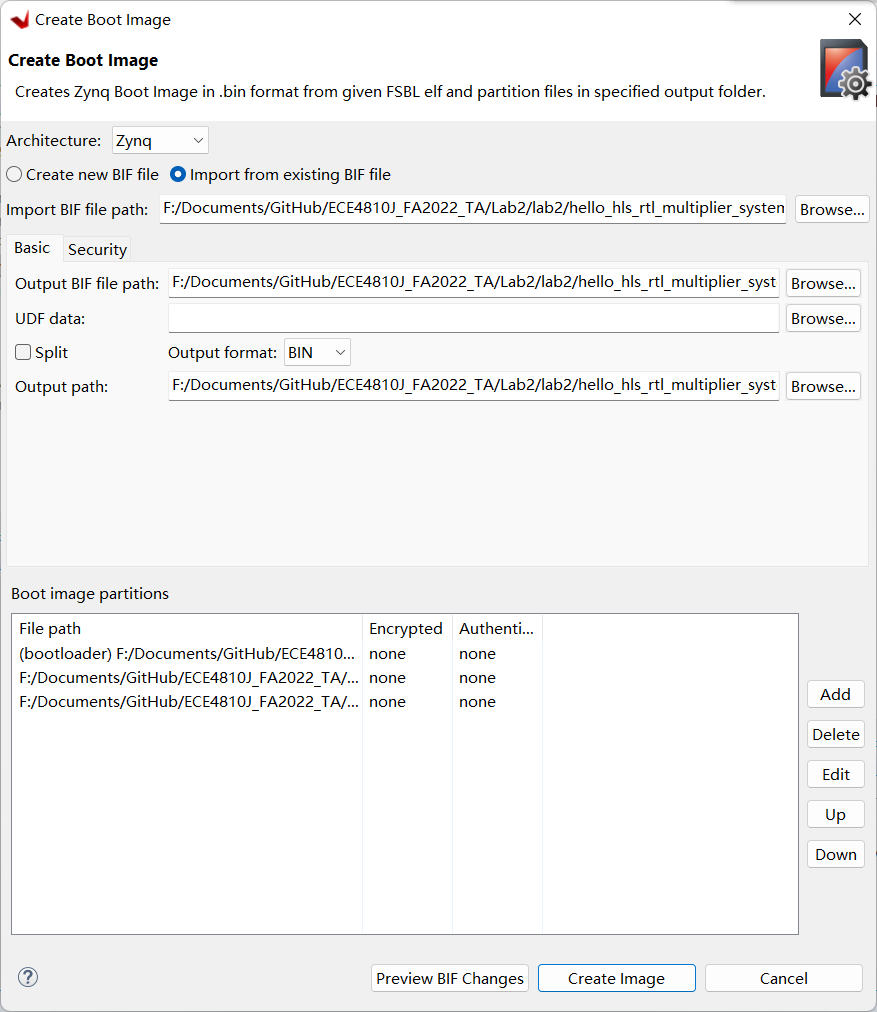
\includegraphics[width=0.8\textwidth]{images/5.png}
    \end{figure}
    The Bootgen console shows:
    \begin{minted}[breaklines,breakanywhere]{text}
cmd /C bootgen -image hello_hls_rtl_multiplier_system.bif -arch zynq -o \
F:/Documents/GitHub/ECE4810J_FA2022_TA/Lab2/lab2/hello_hls_rtl_multiplier_system/_ide/bootimage/BOOT.bin 


****** Xilinx Bootgen v2022.1.2
  **** Build date : Aug  5 2022-23:12:34
    ** Copyright 1986-2022 Xilinx, Inc. All Rights Reserved.

[WARNING]: Partition fsbl.elf.0 range is overlapped with partition Zynq_CPU_wrapper_hw_platform_4.bit.0 memory range
[WARNING]: Partition Zynq_CPU_wrapper_hw_platform_4.bit.0 range is overlapped with partition hello_hls_rtl_multiplier.elf.0 memory range

[INFO]   : Bootimage generated successfully
    \end{minted}
    \item Plug in your MicroSD card for FPGA in your computer with a MicroSD card reader/adapter. Paste the hello\_hls\_rtl\_multiplier\_system/\_ide/bootimage/BOOT.bin file into the MicroSD card.
    \item Plug your MicroSD card back to the FPGA board. Change JP4 from JTAG to SD on Arty Z7.
\end{enumerate}
Now you are ready to observe that the FPGA indeed boots software from the MicroSD card. Connect the FPGA to your PC. If the Vitis Serial Terminal has no response, or does not show "Enter operand A: Performing a test of the RTL\_MULTIPLIER..." and directly show your input number and "Enter operand B:" after your send a number, press PORB (Power-On Reset B) or SRST (external System Reset) used to reset the Zynq without disconnecting and reconnecting the power supply first, because the Arty Z7 does not have a power switch, so when a power source is connected and selected with JP5 it will always be powered on \cite{porb} \cite{porbvssrst} \cite{srst} \cite{ug585}. Make sure a connection via the serial port is established either using the Vitis Serial Terminal or other serial terminals like PuTTY (in PuTTY, change Connection Type to Serial, change Serial Line to your COM port, and change Speed to 115200). Once the FPGA has been connected to your PC via the serial COM port, enter any number through the terminal. The program should start execution, and you should observe that it continually asks the user to enter operands for the RTL/HLS multipliers, respectively, and that it outputs the correct multiplication results. Congrats! Now you know how to boot software from the FPGA’s MicroSD card! Take a screenshot of the Vitis Serial terminal or PuTTY terminal. Note: The same BOOT.bin file can be used to boot from the SPI Flash memory.

% \newpage
\section{Program Python on Arty Z7}\label{S4}
Python is a very powerful and flexible programming language, enabling engineers to perform complex mathematics analysis, implement Artificial Intelligence solutions, and develop a range of other complex engineering solutions. The ability to use Python within the Field Programmable Gate Array (FPGA) space has however previously been limited. With the release of the PYNQ framework, Python developers for the first-time were able to exploit the capabilities and performance provided by programmable logic. While FPGA developers also benefited as they were able to integrate the high-level capabilities of Python with their FPGA designs.

In this lab, we will introduce the PYNQ project. The main goal of PYNQ, Python Productivity for Zynq, is to make it easier for designers of embedded systems to exploit the unique benefits of Xilinx devices in their applications. Specifically, PYNQ enables architects, engineers and programmers who design embedded systems to use Zynq devices, without having to use ASIC-style design tools to design programmable logic circuits. PYNQ achieves this goal in three ways:
\begin{itemize}
    \item Programmable logic circuits are presented as hardware libraries called overlays. These overlays are analogous to software libraries. A software engineer can select the overlay that best matches their application. The overlay can be accessed through an Python API. Creating a new overlay still requires engineers with expertise in designing programmable logic circuits. The key difference however, is the build once, re-use many times paradigm. Overlays, like software libraries, are designed to be configurable and re-used as often as possible in many different applications.
    \item PYNQ supports Python for programming both the embedded processors and the overlays. Python is a “productivity-level” language. To date, C or C++ are the most common, embedded programming languages. In contrast, Python raises the level of programming abstraction and programmer productivity. These are not mutually exclusive choices, however. PYNQ uses CPython which is written in C, and integrates thousands of C libraries and can be extended with optimized code written in C. Wherever practical, the more productive Python environment should be used, and whenever efficiency dictates, lower-level C code can be used.
    \item PYNQ is an open-source project that aims to work on any computing platform and operating system. This goal is achieved by adopting a web-based architecture, which is also browser agnostic. We incorporate the open-source Jupyter notebook infrastructure to run an Interactive Python (IPython) kernel and a web server directly on the ARM processor of the Zynq device. The web server brokers access to the kernel via a suite of browser-based tools that provide a dashboard, bash terminal, code editors and Jupyter notebooks. The browser tools are implemented with a combination of JavaScript, HTML and CSS and run on any modern browser.
\end{itemize}
Please read more details about PYNQ from \href{https://pynq.readthedocs.io/en/latest/}{PYNQ Introduction — Python productivity for Zynq (Pynq)}.

To get started with the tutorial, one must first pick up an Arty Z7-20 as well as a MicroSD card. The first steps involve getting the PYNQ image up and running on the Arty. Once this is complete, the ISO File must be burned to the MicroSD card (which should be at least 8 gigs if possible).
\begin{enumerate}
    \item Here is a list of PYNQ images that correspond to different boards, please choose the PYNQ-Z1 image. \url{http://www.pynq.io/board.html}.
    \item To burn the ISO image to the SD card, you can use imager tools like \href{https://sourceforge.net/projects/win32diskimager/}{Win32 Disk Imager}.
    \begin{figure}[H]
        \centering
        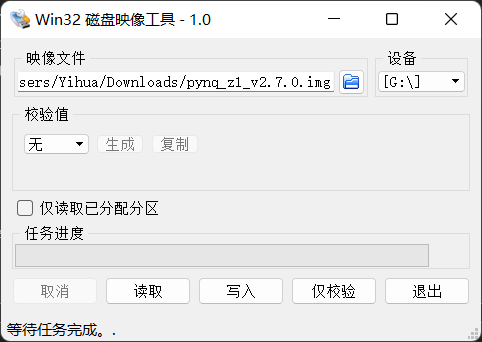
\includegraphics[width=0.6\textwidth]{images/6.png}
    \end{figure}
    \item Once the image is written to the MicroSD Card, it is time to plug the card into the Arty Z7-20, ensure the configuration jumper is set to boot from SD, and connect an Ethernet cable to your computer before powering it on.
    \item Power on the board, and after tens of seconds the yellow LD10, the green LD8 and L9 blinking, you will see the Done LD12 illuminates, indicating the Xilinx Zynq has been configured, followed by activity on the Ethernet LEDs. Once the boot sequence is complete, and the PYNQ framework is ready. The four LEDs and two RGB LEDs will flash several times before leaving the four LEDs illuminated.
    \begin{figure}[H]
        \centering
        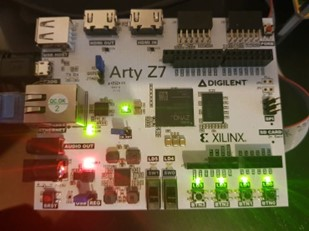
\includegraphics[width=0.7\textwidth]{images/7.jpg}
    \end{figure}
    \item We are now ready to leverage Python on Arty Z7-20, we do this by using Jupyter notebooks running on the Arty Z7-20. To connect to the Arty Z7-20 and its Jupyter notebooks, we need to open a browser on the same network as the Arty Z7-20, entering the address pynq:9090 this will open the initial page as shown below. It is from here that we can develop our Python-based applications. If you cannot open pynq:9090 because of HTTP errors like 500 or 503, see Appendix \ref{A2}.
    % \begin{figure}[H]
    %     \centering
    %     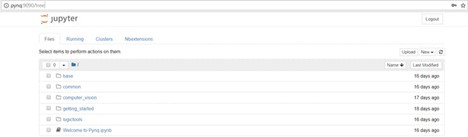
\includegraphics[width=\textwidth]{images/8.jpg}
    % \end{figure}
    \item Take a screenshot of the Jupyter Notebook including the address bar of your browser. Once on the landing page, open the getting\_started directory and read the information on the Jupyter notebooks, Python environments, and advanced Python features. These will provide a great introduction to how to get started using the development environment.
    \item While the Linux image with its Jupyter notebooks and Python run on the processor cores of the Zynq, the programmable logic is used to provide several interfaces and programmable logic overlays. These overlays can be loaded and used from within the Jupyter environment as your Python script executes. The PYNQ image comes with a base overlay that supports all the inputs and outputs (IO) on Arty Z7-20.
    \begin{figure}[H]
        \centering
        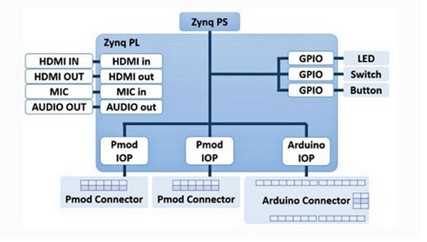
\includegraphics[width=\textwidth]{images/9.jpg}
    \end{figure}
    \item Of course, it is possible to develop custom overlays. These custom overlays are developed using either a traditional flow of Vivado Design Suite including SDK and High-Level Synthesis using Vivado HLS or SDSoC Development Environment. To enable integration within the Python environment, the software (SW) drivers for the programmable logic (PL) are exploited using Python’s C Foreign Function Interface.
\end{enumerate}

\section{(Optional) Optimize Your RTL ALU by Pipelining}\label{Sopt1}
In Section \ref{S2}, you probably simply implement multipliers and dividers in a single clock cycle, the timing violation will be serious, and a huge amount of programmable logic will cost, thus, you will need to pipeline your multiplier and divider in order to derive more acceptable performance, but you do not need to achieve the optimal pipelined performance.

In this section, you are expected to create and package a new IP rtl\_pipe\_alu that combines the pipelined multiplier and divider with the RTL ALU you wrote in Section \ref{S2}. Add it into a block design together with your previously created and packaged IP hls\_alu and the ZYNQ7 Processing System. Make an HDL wrapper, generate the bitstream, take a screenshot of the Implemented Design highlighting RTL ALU and HLS ALU leaf cells, take a screenshot of the Utilization Summary and the Design Timing Summary of the Implemented Design, compare them with the implemented design of the RTL ALU in Section \ref{S2}, export the hardware XSA, create a Vitis application project using the XSA, write an application for testing multiplication and division, build the project, run the project, take a screenshot of the Vitis Serial Terminal to verify the functional correctness of your pipelined multiplier and divider.

If you feel difficult about writing a pipelined divider on your own, you can try to alternatively replace your current design of dividers with the Divider Generator IP of Xilinx LogiCORE IP Product.

\section{Post-lab Questions}\label{SPost}
\begin{enumerate}
    \item What was the resource utilization of the RTL implementation vs. HLS implementation? If they are different, can you guess why there are differences?
    \item Imagine that you have to create an IP block implementing ten different sorting algorithms. Would you rather use a hardware description language or High-level Synthesis? Why?
    \item Read more about PYNQ, and answer the following questions:
    \begin{itemize}
        \item What is a Jupyter notebook? Why do we use it?
        \item What are overlays? What are the benefits of using overlays?
        \item Please list available overlays on the Arty Z7 board.
        \item Comparing part 2 where you design with C/C++ vs. part 4 (PYNQ framework with python), what are the major differences?
    \end{itemize}
\end{enumerate}

\newpage
\section{Deliverables}
Group Deliverables (Compile everything as a single pdf report besides the code):
\begin{itemize}
    \item Section \ref{S2}:
    \begin{itemize}
        \item the screenshot of the Implemented Design highlighting RTL multiplier and HLS multiplier leaf cells
        \item the screenshot of the Utilization Summary and the Design Timing Summary of the Implemented Design
        \item the screenshot of the Vitis Serial Terminal of hello\_hls\_rtl\_multiplier Vitis project
        \item the screenshot of the Synthesis Summary Report of hls\_alu containing Timing Estimate and Performance \& Resource Estimates
        \item the screenshot of the generated Cosimulation Report for hls\_alu
        \item the screenshot of the resource utilization of the Implemented Design highlighting RTL ALU and HLS ALU leaf cells
        \item the screenshot of your Vitis IDE window at the build-finished state of hello\_hls\_rtl\_alu Vitis project
        \item the screenshot of the Vitis Serial Terminal of hello\_hls\_rtl\_alu Vitis project
        \item the code rtl\_alu.sv for Vivado Design Source
        \item the code hls\_alu.cpp for Vitis HLS Source
        \item the code test\_hls\_alu.cpp for Vitis HLS Test Bench
        \item the code hls\_rtl\_alu.c for Vitis Application Project hello\_hls\_rtl\_alu src
    \end{itemize}
    \item Section \ref{S3}: the screenshot of the Vitis Serial terminal or PuTTY terminal
    \item Section \ref{S4}: the screenshot of the Jupyter notebook including the address bar of your browser
    \item Section \ref{Sopt1}:
    \begin{itemize}
        \item the screenshot of the Implemented Design highlighting RTL ALU and HLS ALU leaf cells
        \item the screenshot of the Utilization Summary and the Design Timing Summary of the Implemented Design
        \item the screenshots of the Vitis Serial Terminal of pipe\_hls\_rtl\_alu Vitis project
        \item the code deliverables are the same as Section \ref{S2}; if you finish this part, submit your code used for this section instead of the code for Section \ref{S2}
    \end{itemize}
    \item Section \ref{SPost}: answers
\end{itemize}
\section{Grading policy}
\begin{table}[H]
    \centering
    \begin{tabular}{|c|c|}
        \hline
        Factors & Percentage \\
        \hline
        Section \ref{S2} & 45\% \\
        \hline
        Section \ref{S3} & 20\% \\
        \hline
        Section \ref{S4} & 20\% \\
        \hline
        Section \ref{Sopt1} & 20\% (bonus) \\
        \hline
        Section \ref{SPost} & 15\% \\
        \hline
    \end{tabular}
\end{table}

\newpage
\appendix
\section{Peer Evaluation Form}
\begin{table}[H]
    \centering
    \begin{tabular}{|c|c|c|c|c|}
        \hline
        Part & Your work & Your partner's work & Your score & Your partner's score \\
        \hline
        Section \ref{S2} & & & & \\
        \hline
        Section \ref{S3} & & & & \\
        \hline
        Section \ref{S4} & & & & \\
        \hline
        Section \ref{Sopt1} & & & & \\
        \hline
        Section \ref{SPost} & & & & \\
        \hline
    \end{tabular}
\end{table}

\section{Troubleshooting}\label{A2}
\subsection{PYNQ HTTP Connection}
If you could not connect to the pynq after you have set up your board and LEDs illuminate properly, you should do the following configuration:

Quit any VPN connections and proxy connections. For Windows 10/11, go Control Panel->Network and Internet->Network and Sharing Center->View your active networks->Access type: Internet, Connections: WLAN (or the network you are currently connecting, since you may connect the board and your computer by a cable, you are probably using WLAN)->Properties \cite{pynqhttp}. In the pop-up window <network\_name> Properties, go tab Sharing, in the Internet Connection Sharing frame, check "Allow other network users to connect through this computer's Internet connection", and for Home networking connection: Select a private network connection, select the proper connection (usually it is ethernet). Refresh pynq:9090, you will be able to connect. The password is \texttt{xilinx} by default.
\begin{figure}[H]
    \centering
    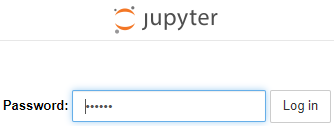
\includegraphics[width=0.5\textwidth]{images/10.png}
\end{figure}

\printbibliography
\end{document}

